% !TEX encoding = UTF-8
% !TEX program = pdflatex
% !TEX root = InformationRetrieval.tex
% !TEX spellcheck = it-IT

\chapter{Web search}

La principale differenza tra i documenti puramente testuali e quelli web è che la collezione di documenti non è nota a priori.
Inoltre, per i file testuali, avevamo un identificativo univoco per ciascun documento e ogni volta che andavamo a fare reperimento, fornivamo in risposta dei documenti diversi, mentre nell'ambito web possono esserci due pagine con lo stesso contenuto.
In più le pagine web sono costruite con dei linguaggi di mark-up che forniscono delle informazioni che permetto di costruire degli \textbf{authority file} per distinguere quale pagine sono state create da delle persone autorevoli.
Un'ulteriore differenza sta nel fatto che i documenti web possono essere tra loro linkati, cosa che non avviene per i documenti testuali.

\section{Il contesto Web}

La collezione di documenti è costituita da una collezione di pagine web che possono essere o documenti HTML o documenti multimediali (PDF, JPEG, MP3, ecc.).

Per quanto riguarda le pagine web si possono sfruttare gli hyperlink per ottenere informazioni aggiuntive relative ai documenti.
Questi hyperlink possono essere sfruttati dai \textbf{web crawler}, programmi che navigano sul web per indicizzare le pagine.
L'esecuzione di questi programmi deve essere continua, perché il web è un ambiente dinamico e anche il contenuto delle pagine già indicizzate può cambiare.

Inoltre le pagine web sono composte da un header che contiene dei meta-tag che, se usati correttamente, descrivono il contenuto della pagina web, fornendo informazioni come l'autore, la data dell'ultimo aggiornamento, ecc.

Per quanto riguarda le query effettuate dagli utenti, tipicamente sono corte, composte da poche parole e l'utente tipo è impaziente: guarda solo i primi risultati della ricerca.

I link presenti nelle pagine web possono essere assoluti o relativi. Quelli assoluti possono riferire anche altri siti web, mentre quelli relativi riferiscono altre pagine interne del sito.
In base alla tipologia di reperimento che si può scegliere se fermarsi ad indicizzare solo l'homepage del sito, oppure proseguire ad analizzare anche le pagine interne.
Ad esempio Google è un motore di ricerca generalista, che può essere utilizzato per qualsiasi tipo di query, quindi la sua indicizzazione deve essere molto ampia. Se invece c'è un motore di ricerca specialistico sulla filosofia orientale, ci si può accontentare di indicizzare tutte le pagine di un sotto-insieme (ampio) di siti web, considerando tutte le pagine interne.

\begin{figure}[htbp]
	\centering
	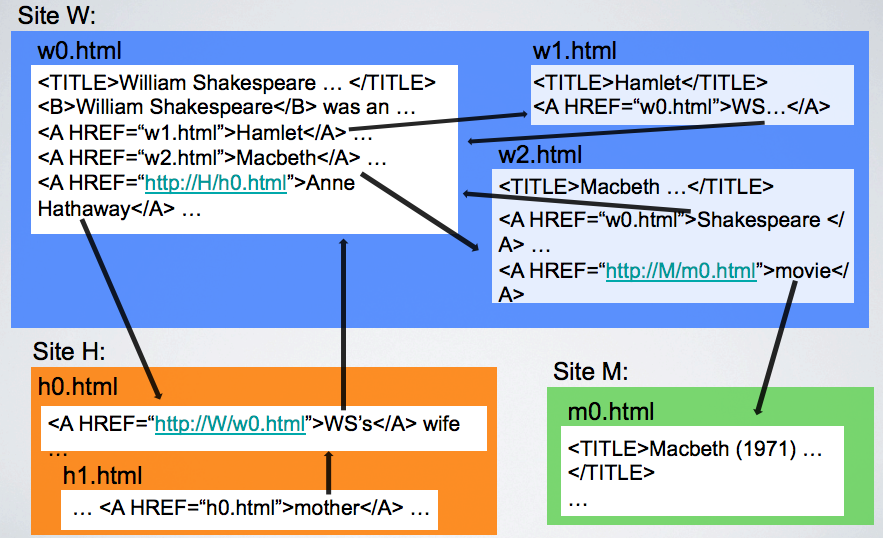
\includegraphics[width=0.5\textwidth]{images/l17-fig-1.png}
\end{figure}

Infine ci sono dei problemi legati all'autorevolezza e qualità delle pagine che non sempre è garantita, inoltre, la popolarità di una pagina non può essere usata come indice della sua qualità, perché potrebbe essere una pagina di spam.

\section{La struttura del Web}

Il web nasce con il contesto di iper-testo, ovvero con l'idea di poter consultare documenti che sono correlati tra di loro. Se un documento non ha dei collegamenti dall'esterno, questo non è accessibile.

\begin{figure}[htbp]
	\centering
	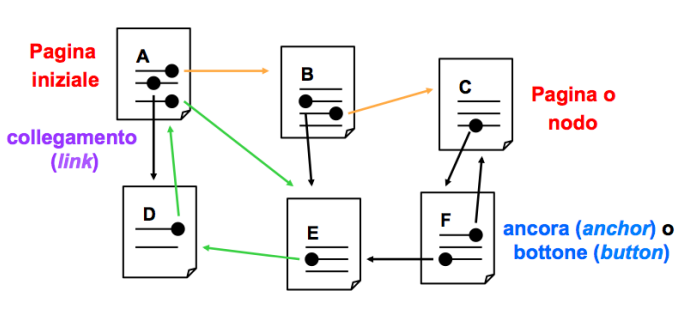
\includegraphics[width = 0.5\textwidth]{images/l17-fig-2}
\end{figure}

Un po' di terminologia:

\begin{itemize}
	\item \textbf{Pagina} o \textbf{nodo}: sinonimi che indicano un elemento o documento unitario dell'ipertesto che può essere utilizzato da un utente finale nella consultazione o navigazione. \`E una singola porzione atomica dell'ipertesto.
	\item \textbf{Ipertesto}: documento complesso organizzato con una struttura reticolare.
	\item \textbf{Collegamento} o \textbf{link}: le singole e diverse parti di un ipertesto sono organizzate in modo indipendente, poi vengono collegate fra di loro attraverso dei collegamenti o rimandi denominati link, che guidano il fruitore dal un nodo all'altro. Da notare che a livello implementativo i collegamenti non esistono, vengono infatti implementati utilizzando degli indirizzi per riferire i vari nodi.
	\item \textbf{Ancora} o \textbf{bottone}: il simbolo che indica al fruitore che da una specifica porzione di un nodo è stato attuato un collegamento con un altro nodo.
\end{itemize}

L'insieme delle pagine web e dei vari collegamenti può essere rappresentato come un grafo orientato (\textbf{web graph}) dove ogni nodo rappresenta una pagina e c'è un arco diretto tra un nodo ed un altro solo se c'è un collegamento che da una pagina va all'altra.
Ovviamente questo grafo è dinamico in quanto l'insieme delle pagine web è in continua evoluzione.

La modellazione come grafo è utili per formalizzare alcune misure della rilevanza, come il PageRank.

\begin{figure}[htbp]
	\centering
	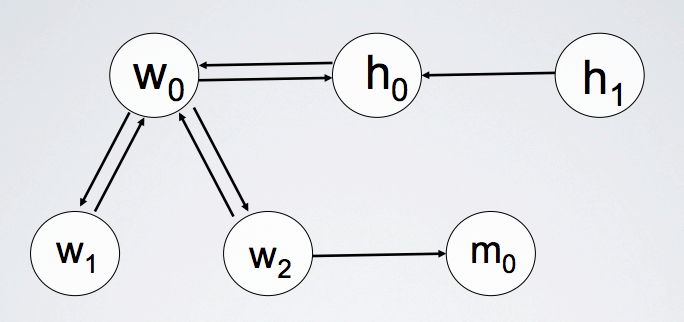
\includegraphics[width = 0.5\textwidth]{images/l17-fig-3}
\end{figure}

Le pagine presenti nel web possono essere:

\begin{itemize}
	\item \textbf{Statiche}: il contenuto della pagina è preparato e reso disponibile prima di una qualsiasi richiesta di un browser (o crawler).
	\item \textbf{Dinamico}: il contenuto della pagina è generato al momento della richiesta e dipende in parte dalla tipologia di richiesta effettuata e dal momento in cui questa viene fatta.
\end{itemize}

Per un crawler questa differenza non è importante per discriminare il contenuto della pagina, perché alla fine quello che interessa sono le informazioni presenti, non come la pagina viene generata.
Tuttavia bisogna tenere in considerazione che il contenuto di una pagina dinamica può cambiare nel tempo.

\subsection{Il web nascosto}

Molte pagine web fanno parte del \textbf{deep web}, ovvero una porzione di internet che non è normalmente raggiungibile perché le pagine al suo interno non sono \textit{puntante} da link presenti in altre pagine, oppure perché sono protette da password, oppure perché sono su server accessibili solamente all'interno di una rete privata. Un altro esempio di queste pagine sono quelle che vengono generate in risposta ad una determinata query.

Tutte queste pagine possono avere contenuti interessanti per un crawler, ma tipicamente è impossibile indicizzarle.

\subsection{La dimensione del web}

Data la sua dinamicità è difficile stimare la dimensione effettiva, inoltre, possono esserci pagine con contenuti di interesse limitato e altre molto più interessanti.

Se ci si limita a queste ultime, la dimensione del web può essere stimata considerando l'\textbf{Indexable Web} (\textbf{IW}) pubblico, ovvero quella parte di web che è indicizzata dai principali motori di ricerca, sia generalistici che specialistici.

La necessità di stimare la dimensione del web deriva dal fatto che è utile per stimare:

\begin{itemize}
	\item il tempo necessario alla raccolta delle pagine web d'interesse.
	\item la banda necessaria ad acquisire i vari documenti. Questi documenti possono trovarsi sparsi per il mondo, in zone con una connessione ad internet limitata.
	\item la quantità di memoria necessaria alla gestione e funzionamento del motore di ricerca.
\end{itemize}





















